\documentclass[12pt, letterpaper]{article}
\usepackage[utf8]{inputenc}
 \usepackage[letterpaper, margin=0.8in]{geometry}
 \usepackage{amssymb}
\usepackage{amsmath}
 \usepackage{enumitem}
\usepackage {listings}
\usepackage{pgfplots}
\usepgfplotslibrary{external}
\usepackage{graphicx}

\title{CS425 Project 4(Report)\\Back-Propogation}
\author{Ksenia Burova}
\date{November \(20^{th}\), 2017}

\begin{document}
\maketitle

\noindent {\bf Abstract:} In this project, the goal was to implement and examine multilayer artificial neural networks (ANNs) and explore back-propagation learning algorithm by applying it to spam classification problem. The task was simply to classify given data instances as spam or not. After implementing training and testing functions, we had to make observations on how different parameters for building networks, like number of hidden layers, number of nodes (neurons), number of epochs and learning rate would affect training, validation and testing performance. For extra credit, we observed how data dimensionality reduction would influence training results. For performance analysis results were displayed in several plots.

\begin{enumerate}[label=\Roman*.]
 
 	{\bf \item Back-Propogation.} \\
	
 	Perceptron, pattern classification device, is a great example of feed-forward neural net. \\
	{\center 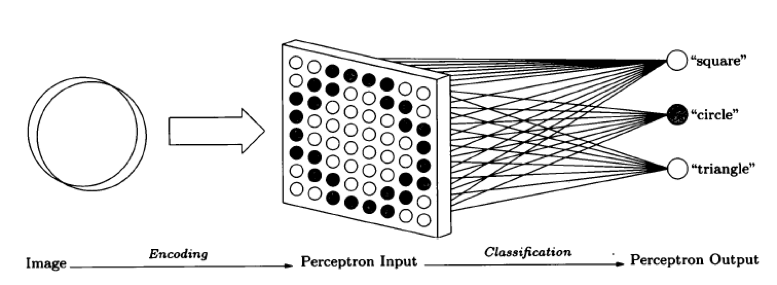
\includegraphics[scale=1]{1.png} \\}
	Perceptron demonstrates how image encoding and classification goes one direction. here are single-layer and multiple-layer perceptron kinds of neural network. Single-layer one have inputs and outputs only, whereas multiple-layer also have one or more hidden layers in between.\\
	
	Back-propagation algorithm is the most commonly used for training multi-layer neural networks. The general idea behind this algorithm is run several data sets, compare output with expected value and compute the predefined error function. Then error function is fed back through the network and used for adjustment of all the weights to minimize the value of the error function. Such operation is done several number of times until error is minimized to almost zero value, which indicates that network is trained and should solve testing problems correctly. Let's look at the example with using logistic sigmoid for output layer, since we have 2-class problem, it is 0 or 1 for no spam or spam respectively:
	{\center 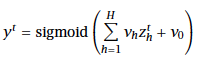
\includegraphics[scale=0.5]{7.png} \\}
	
	So, as it's been said, first we propagate input values forward through the network:
	{\center 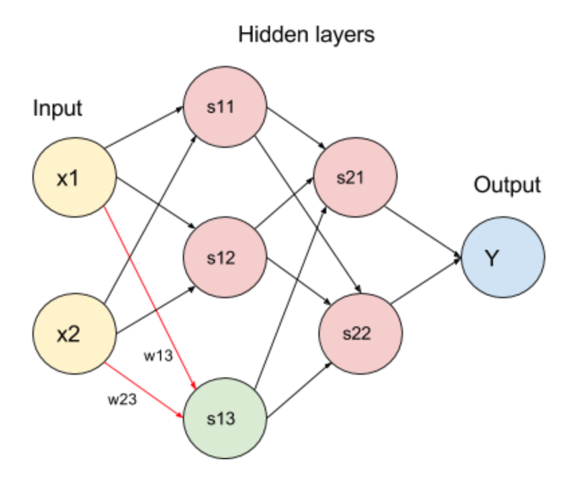
\includegraphics[scale=.9]{2.png} \\}
	
	Next, we start with two inputs and propagate through two hidden layers before calculating the output. We calculate sigmoidal function \(g(x) = \frac{1}{1 + exp(-x)}\) value for each node, where \(x\) is determined by summation of products of all weights (coming into a node) and \(s_{ij}\) values from previous layer corresponding to those weights. We also add bias weight to it for weigh correction. So, we get \( x_k = \sum\limits_{i=0}^{prevNodesNum} s_{ij}w_{ik}+b_k \). So, in our example, we do \(x = x_1w_{13} + x_2w_{23} + biasWeight\). And then calculate \(g(x)\) for node colored in green, which is sigma value that is used in calculations for nodes in next layer. \\
	
	{\center 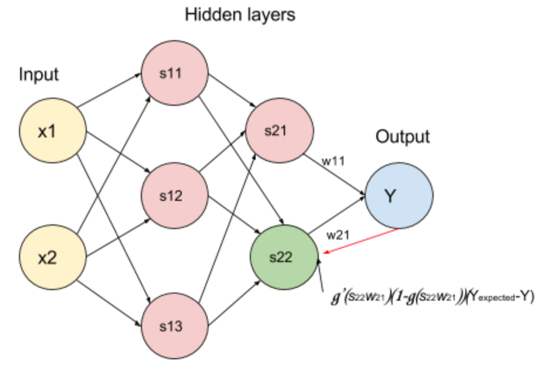
\includegraphics[scale=1]{3.png} \\}
	{\center 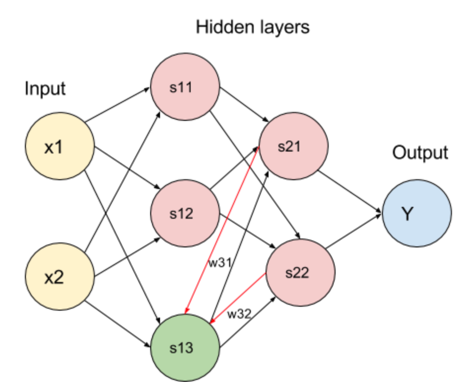
\includegraphics[scale=1]{4.png} \\}
	
	After output is computed, we calculate the error function \(\delta\) value. First layer in the end will take in account the difference between expected output and received one. And for every other node, we calculate \( \delta_{s_{ij}} = g'(x_{ij})\sum_kw_{kj}\delta_{s_{i+1,j}} \). As we can see, delta function is from layer before is used for calculation of delta function for current node. Calculating the derivative of the sigmoidal function gives us information about how the output changes when the input changes. If its value is too large that means the input was near its threshold and little change may change  \(g(x)\), if it's too small, then value of \(g(x)\) is really close to 0 or 1. Also, the sign of \(g'(x)(t-y)\) will tell us which way neuron was wrong. Overall, this term will give us all the information needed for error correction. We use delta function and learning rate value for computing adjusted weight.
	{\bf \item Project Data.} \\
	
	 In this project, we were given a file {\it spambase.data} which had 58 attributes:
	 \begin{itemize}
	 	\item 48 continuous real [0,100] attributes of type word\_freq\_WORD (percentage of words in the e-mail that match WORD)
		\item 6 continuous real [0,100] attributes of type char\_freq\_CHAR (percentage of characters in the e-mail that match CHAR)
		\item 1 continuous real [1,...] attribute of type capital\_run\_length\_average (average length of uninterrupted sequences of capital letters)
		\item 1 continuous integer [1,...] attribute of type capital\_run\_length\_longest (length of longest uninterrupted sequence of capital letters)
		\item 1 continuous integer [1,...] attribute of type capital\_run\_length\_total (total number of capital letters in the e-mail)
		\item Class: (0 - no spam, 1 -  spam)
	\end{itemize}
	
	There were no missing values in data but data values range is different for some attributes. Because of that I decided to normalize data. Without standardization my program would fail to run or would give me really bad results.
	I've placed all continuous values of the data into multidimensional array called {\bf dataFeatures}, and kept classes in one-dimensional array called {\bf dataLabels} for simplicity of implementation. During experiments, data was split into 3 sets: training, validation and testing. I used 50/25/25 proportion rule for splitting the data. 
		
	{\bf \item Tools and Program.}\\
	
	I've used {\bf python} programming language, {\bf numpy} library for arithmetic, {\bf sklearn} library for splitting my data into training, validation and testing datasets, and {\bf matplotlib} library to built plots for this project. I have a program named {\bf abckprop.py} , that includes 2 classes: {\bf Data} for normalizing and constructing data sets, and {\bf BackProp} that has back propagation implementation. I've split the algorithm into several functions:
	\begin{itemize}
		\item compute\_outputs(): forward propagation
		\item compute\_delta(): consruct delta for back propagation
		\item update\_weights(): propagate backwards
		\item train\_network()
		\item validate\_network()
		\item test\_network()
		\item plot\_RMSE()
		\item plot\_accuracy()
		\item run(): for given number of epochs it trains and validates network, saves rmse (see below) values for each epoch, plots results and tests network
	\end{itemize}
	
	In my {\bf Data} class I have {\it reduce(k)} function that I can use to reduce dimensions of the data to k PCAs. My {\it split()} function takes features array as argument for splitting data into 3 sets, I pass {\it Z} when use reduced data, and just {\it self.features}, when I need to use my original data.\\
	
	I use {\bf main.py} to create instances of my classes to run experiments, where I specify parameters by hand.\\
	
	{\bf \item Performance metrics.}\\
	
	As measure of the differences between values I'll be using root-mean-square error (RMSE):
	{\center 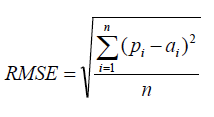
\includegraphics[scale=0.5]{6.png} \\}
	When I test my network, I allow (last rmse + 0.01)  difference between my and expected results. If difference is higher I mark it as incorrect prediction. \\
	
	To evaluate performance of  classification algorithms, we have to compare correct classifications with our classifications on evaluation data sets after algorithm is run. We are going to calculate and look at some of the following values: 
	\begin{itemize}
		\item Confusion Matrix \\
		{\center 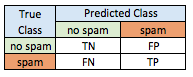
\includegraphics[scale=1]{5.png} \\}
		where TP = \# true positives, TN = \# true negatives, FP = \# false positives, FN = \# false negatives.\\
		\item Accuracy = (TN + TP) / (TN + TP + FN + FP)\\
		{\bf Accuracy} tells us what percent of data was classified correctly. \\
		\item TPR (true positive rate, recall, or sensitivity) = TP / (TP + FN)\\
		{\bf Sensitivity} shows us rate at which true positives are not missed/overlooked \\
		\item PPV (positive predictive value or precision) = TP / (TP + FP)\\
		{\bf Precision} is basically a fraction of relevant positive data from all the positive data we have, meaning have many of those classified as spam are really spam e-emails. \\ 
		\item TNR (true negative rate or specificity) = TN / (TN + FP)\\
		{\bf Specificity} is a rate that shows how well we can distinguish data that is truly negative, meaning that e-mail is not spam.\\
		\item F Score = PPV * TPR / (PPV + TPR)\\
		{\bf F score} is a harmonic average of precision and sensitivity, it is basically used if we can't decide with of 2 metrics to use for performance measurements. \\
	\end{itemize}
	 I mainly be looking at accuracy in my observations, but my {\bf results.txt} output file will contain all the other results.\\
	 
	{\bf \item Experiment Observations. }\\
	
	In general, the goal of the project was to experiment with different number of layers and neurons within each layer, different number of epochs and learning rates. For each epoch we had to train our network on training data set and calculate RMSE error by checking performance on validation set. \\
	We use online learning, meaning that we write the error function on individual instances. Starting from random initial weights, at each iteration we adjust the parameters a little bit to minimize the error, without forgetting what we have previously learned.
	
	In my main function, I've listed following layer-neurons , epochs and learning rate combinations:
	\begin{verbatim}
	    layers = [ [15],
              [65],
              [100],
              [70, 70],
              [30, 30],
              [60, 70, 80],
              [30, 40, 30],
              [15, 15, 15],
              [10, 10, 10, 10],
              [60, 70, 70, 60],
              [15, 15, 15, 15, 15],
              [60, 70, 100, 70, 60]]
    epochs = 500
    lrate = [0.01, 0.1, 0.25, 0.4, 0.65, 0.85, 1.0]
	\end{verbatim}
	 I mix and match all these to observe different results. I use 500 epochs by default due to runtime. More epochs make all of my combinations run for too long. So I decided to check higher/lower number of epochs after I see what learning rate and layers/neurons combination works the best.\\
	 
	Let's look at the results with one layer.
	{\center 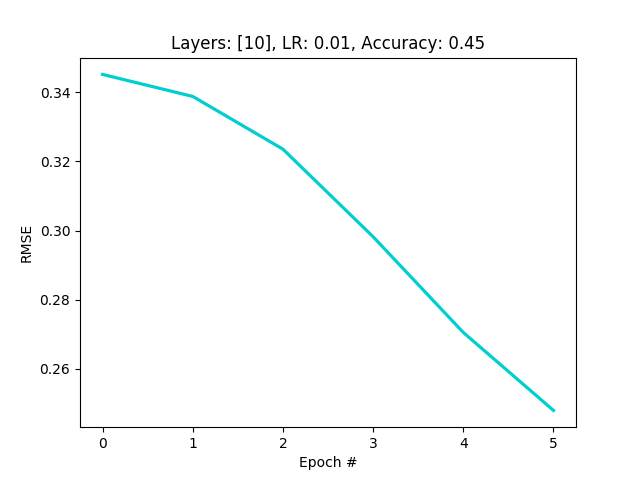
\includegraphics[scale=0.7]{../images/rmse_0.png} \\}
	We can see here for 1 layer with 15 neurons that pretty much all learning rates worked fine except for 0.01, that network has worse results and it took a little bit longer for that network to evolve. The results seem pretty smooth after about 300 epochs.
	{\center 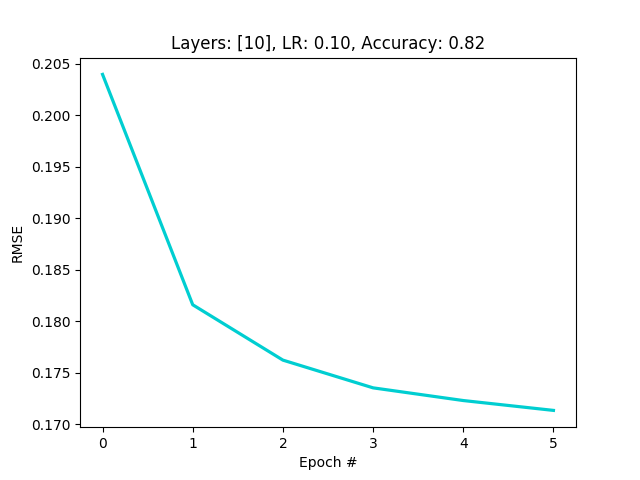
\includegraphics[scale=0.7]{../images/rmse_1.png} \\}
	Adding more neurons, slightly more than number of inputs, makes results a little bit better. But again. optimal number of epochs seems to be about 350, and higher learning rates make accuracy higher.
	{\center 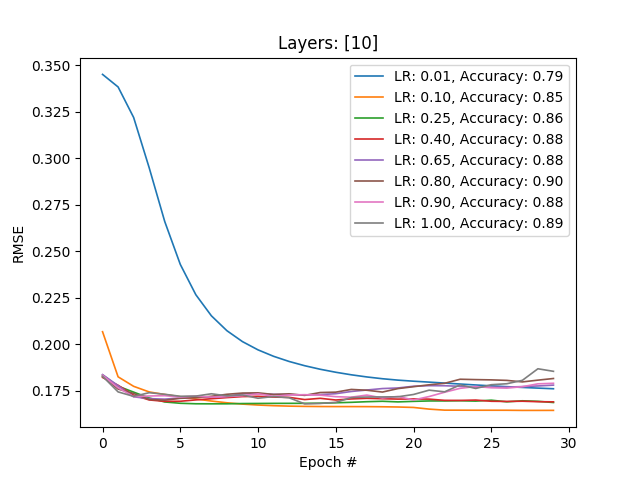
\includegraphics[scale=0.7]{../images/rmse_2.png} \\}
	Adding too many neurons makes results a little noisy. Results are not better than with 65 neurons, so it seems pointless to add too many neurons. Or probably we need to have many more epochs for better results. \\
	
	 Let's look at 2 layers. First experiment has less neurons than number of inputs n each layer.
	 {\center 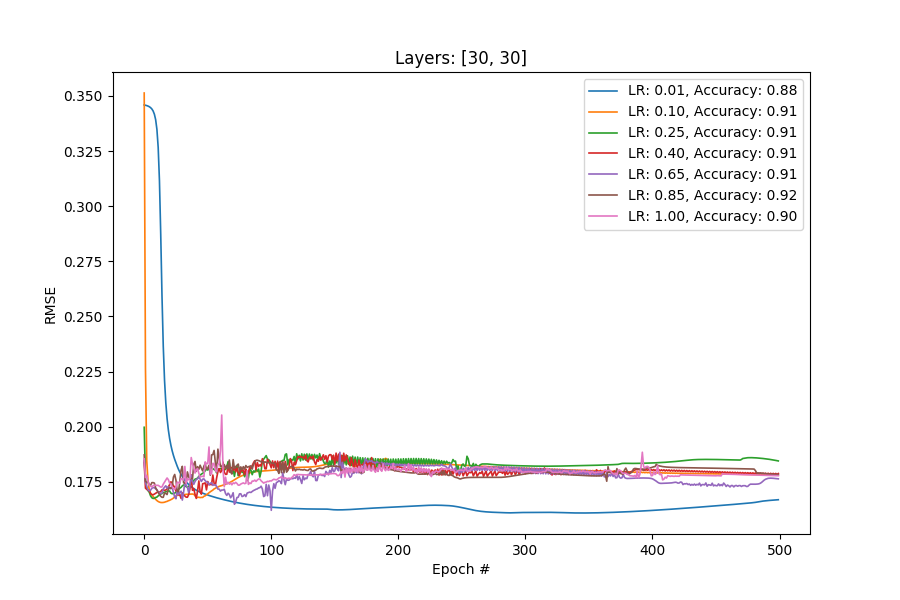
\includegraphics[scale=0.7]{../images/rmse_4.png} \\}
	 Accuracy here is higher than in all 3 results with 1 layer. At about 300-330 epochs rmse value seems to be the most stable and low at the same time for all learning rates. 0.85 learning rate shows the highest prediction accuracy, we might want run this net for more epochs to see what changes we may have in results.\\
	 
	 Having more neurons than number of inputs in each layer seems to have more noise in lower epochs. Accuracy results are better here for all learning rates but we can't tell if higher or lower learning rates are better. We definitely would want to run this net for more epochs or may be stop earlier. It is possible that we are overfitting networks with 0.65 learning rate and higher. \\
	  {\center 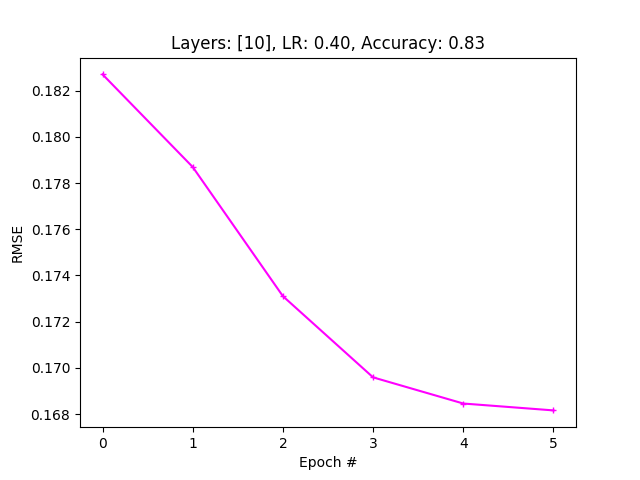
\includegraphics[scale=0.7]{../images/rmse_3.png} \\}
	  I have 3 experiments with 3 layers. First has very low number of neurons.
	  {\center 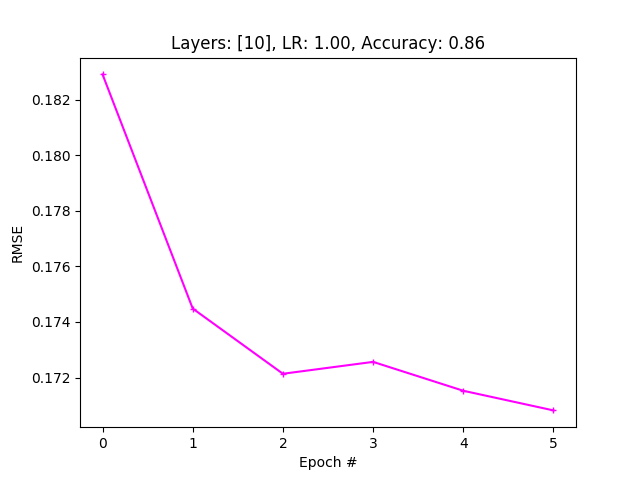
\includegraphics[scale=0.7]{../images/rmse_7.png} \\}
	  
	  Network with learning rate of 0.25 has the highest accuracy so far.  Net with 0.1 learning rate performed worse than in any other experiments. Graph looks very noisy, so I assume  that 500 epochs is not enough for making conclusions with nets that have 3 layers. Net with 0.01 learning rate takes longer to evolve here too than nets with less layers.
	   {\center 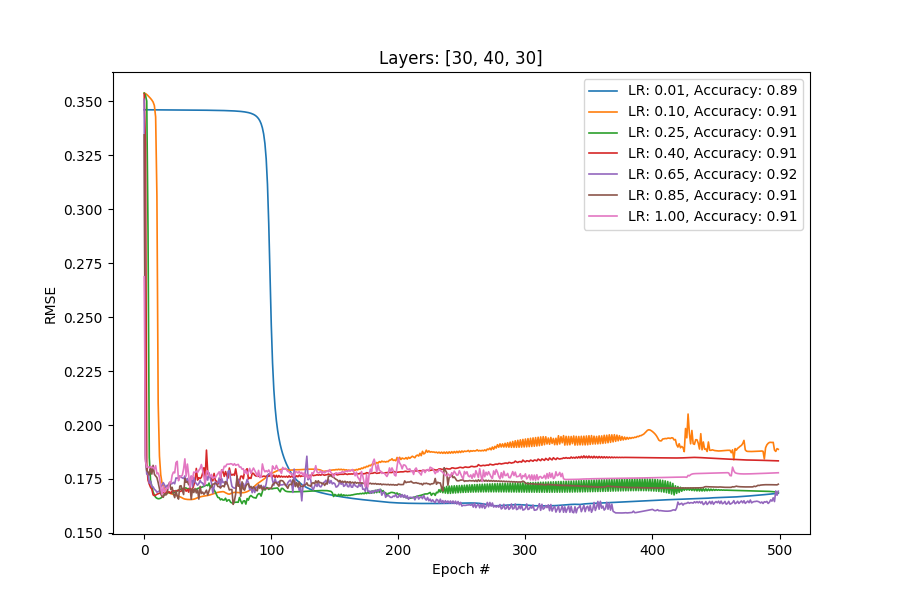
\includegraphics[scale=0.7]{../images/rmse_6.png} \\}
	   Network with a bit more neurons looks very similar. It also has much noise but results seems to be more smooth.
	   {\center 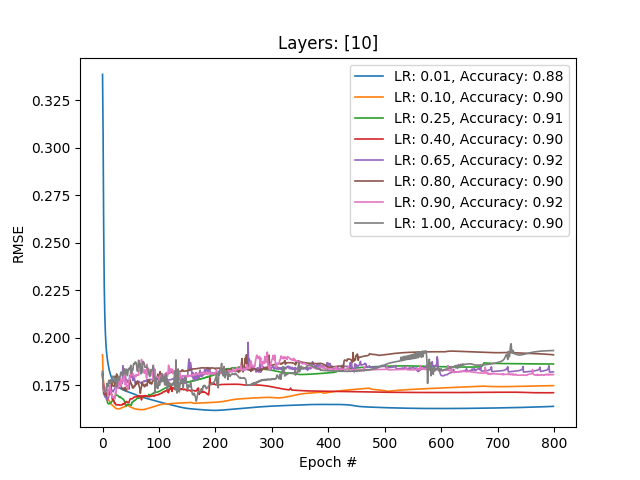
\includegraphics[scale=0.7]{../images/rmse_5.png} \\}
	   Here we might have too many neurons in highest level that makes results undefined a bit. More neurons and layers seem to require more than 500 epochs in general.\\
	    
	   Next I tried 4 layers. First one has smaller number of neurons again.
	   {\center 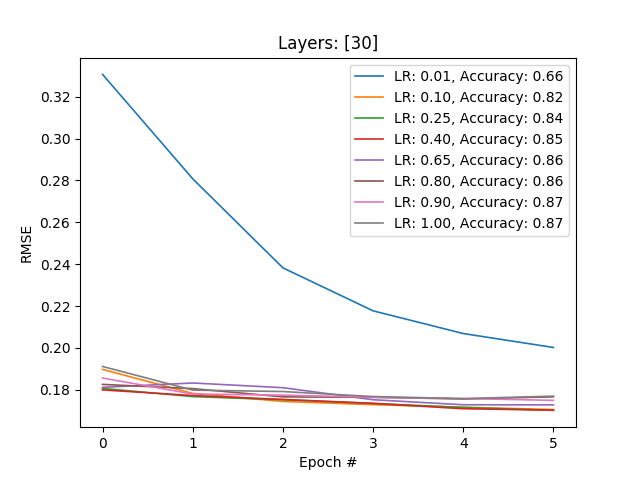
\includegraphics[scale=0.7]{../images/rmse_8.png} \\}
	     
	   We see that one network never evolves at all. Other ones take longer as well than nets with 3 and less layers. Accuracy is fine for all nets that evolved but we could run this example for more epochs I think to see what may happen. RMSE values seems to jump a lot in first 300 epochs.\\
	     
	   Having greater (but not too many) number of neurons in each layer seems to increase performance. But because we may see a lot of jumps in RMSE values I'd give this experiment more epochs to see if results can get even better. \\
	   {\center 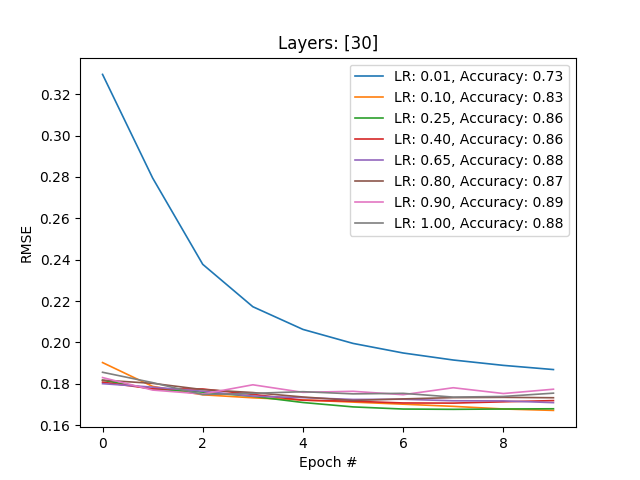
\includegraphics[scale=0.7]{../images/rmse_9.png} \\}
	   Lastly, I looked at nets with 5 layers. I did the same thing here as in other runs. I looked at network with lower number of neurons than number of inputs, and I checked network that has a bit higher number of neurons than number of inputs.
	      
	   {\center 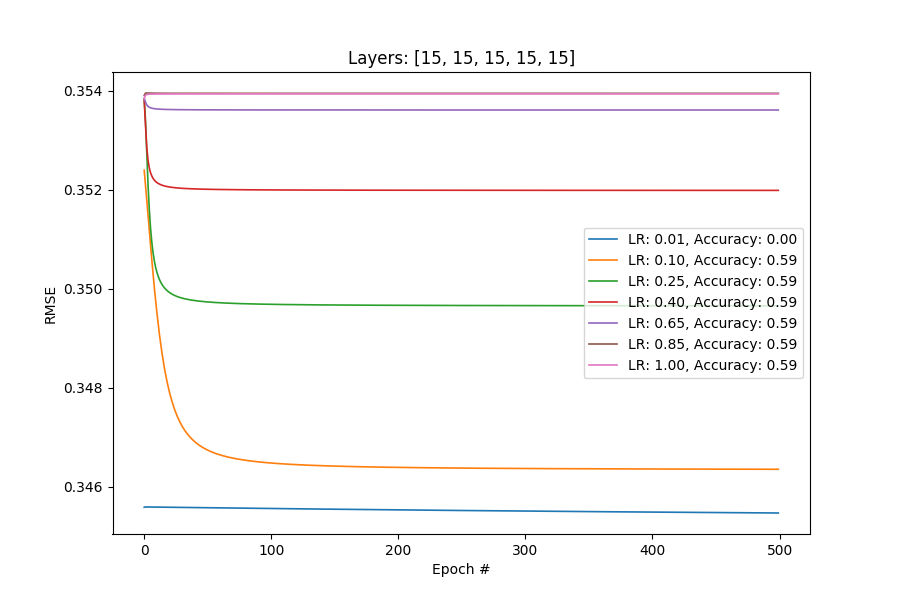
\includegraphics[scale=0.7]{../images/rmse_11.png} \\}
	   We definitely need to run this network for more epochs for all learning rates to discuss any results.
	   {\center 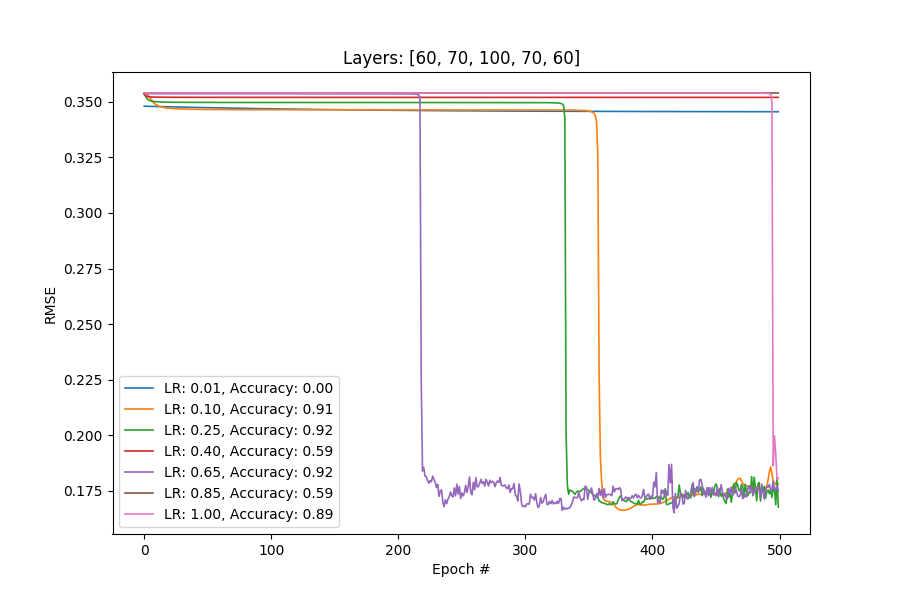
\includegraphics[scale=0.7]{../images/rmse_12.png} \\}
	   Larger number of neurons has much better results, but we still would want to add some epochs since not all nets evolved any way, and there is a lot of jumps in RMSE values for those that have evolved.\\
	      
	   In general, after looking at all runs, it seems better to have more neurons than number of inputs in each hidden layer. With lowering number of layers we might lose some information about input I assume. More layers require higher number of epochs for network to be trained properly.\\
	      
	   In my project, I also decided to look at how accuracy changes for different number of epochs. I chose network with one hidden layer and 65 neurons, net with 2 hidden layers and [70, 70] neurons and another with 5 hidden layers and  [60, 70, 100, 70, 60] neurons, since we looked at these tree already. First lets's look at only 50 epochs.
	   {\center 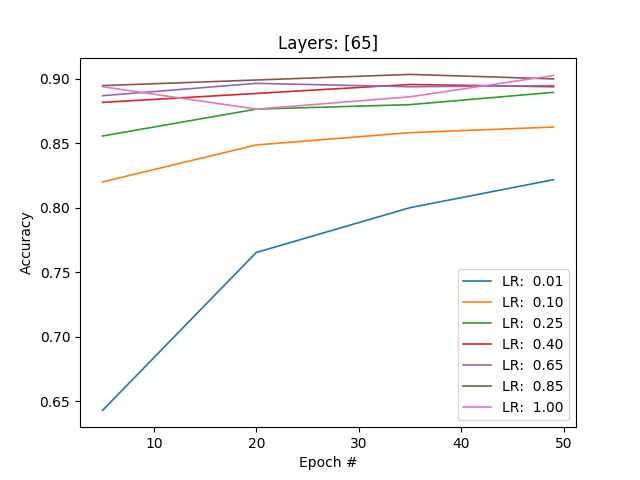
\includegraphics[scale=0.7]{../images/accuracy_0.png} \\}
	   The RMSE distribution looked as following for 50 epochs: 
	   {\center 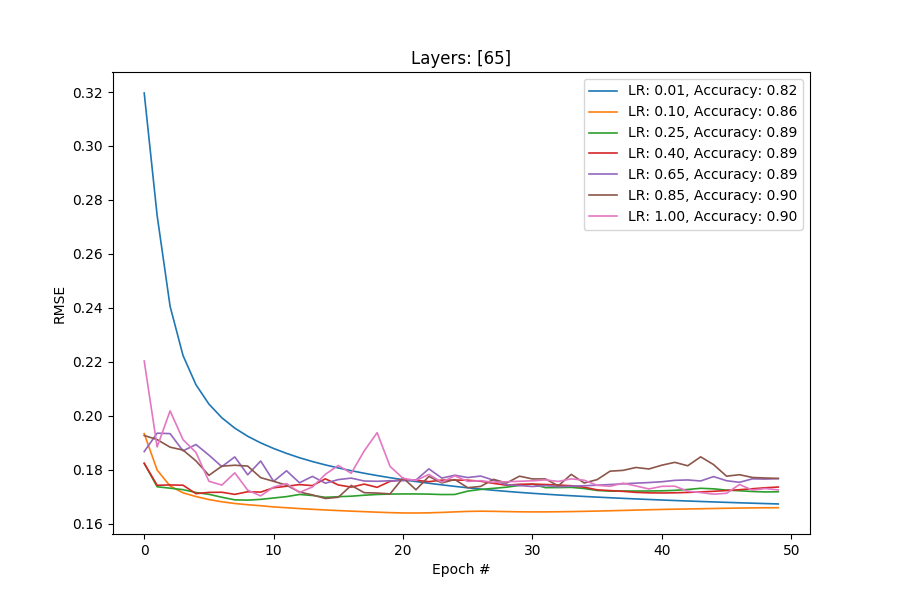
\includegraphics[scale=0.7]{../images/rmse2_0.png} \\}
	          
	   Accuracy  increases with number of epochs for lower learning rates, and is higher in general for higher learning rates. \\
	          
	   For 2 and 5 hidden layers 50 epochs is too small. Accuracy is too low and the same for all learning rates.
	   {\center 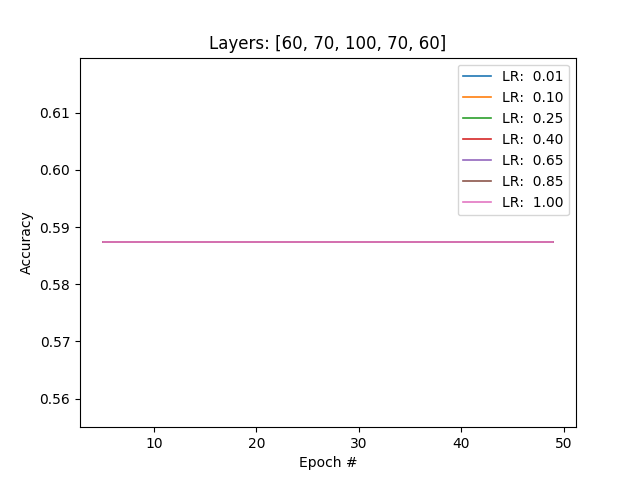
\includegraphics[scale=0.7]{../images/accuracy_1.png} \\}
	           
	   I also ran all 3 networks for 5000 epochs. It seems to be too much for 1 layer.
	   {\center 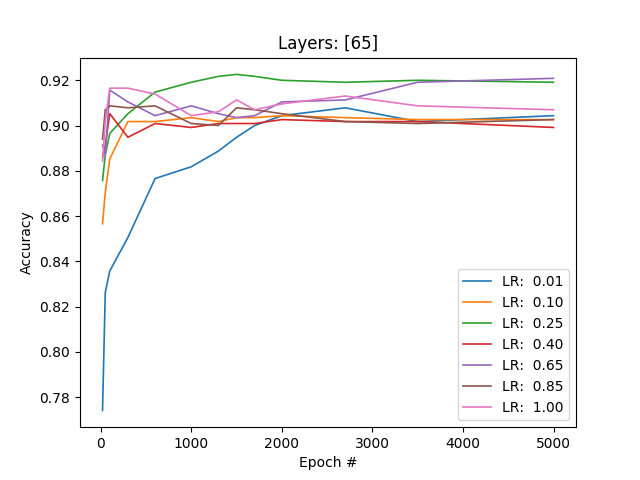
\includegraphics[scale=0.7]{../images/accuracy2_0.png} \\}
	   Accuracy gets a bit higher than 0.92 for net with learning rate of 0.25, but drops after ~1500 epochs, we probably overfit it. 2500-3000 epochs is most optimal for almost all rates.
	    {\center 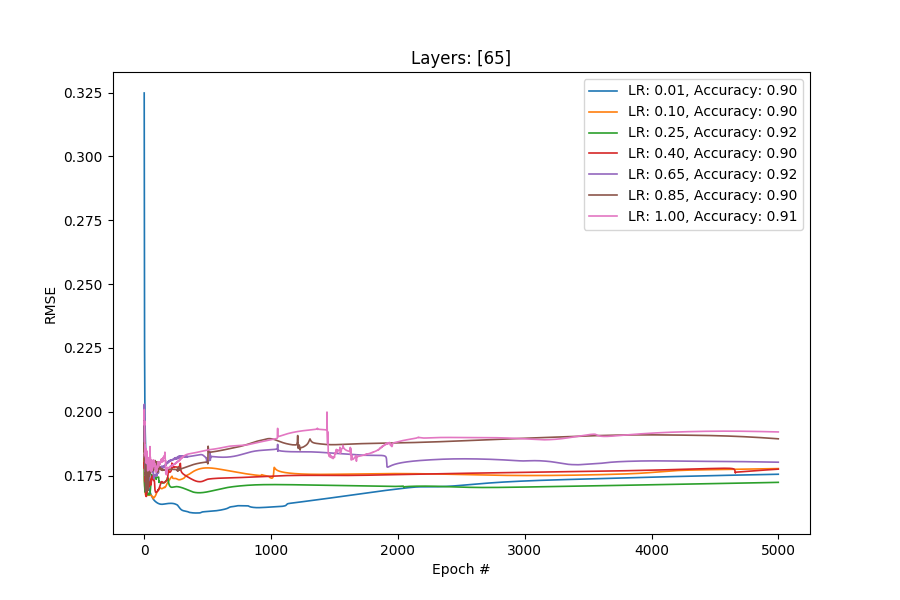
\includegraphics[scale=0.7]{../images/rmse3_0.png} \\}
	    So we are right, RMSE becomes somewhat stable after 2000 epochs.\\
	    
	    With 2 hidden layers 5000 also is too much. We definitely overfit networks after about 1000 epochs.
	     {\center 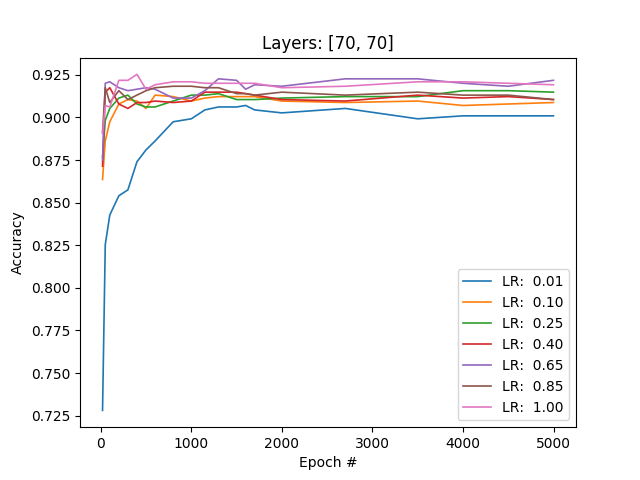
\includegraphics[scale=0.7]{../images/accuracy2_20.png} \\}
	     Net with learning rate of 1.0 seems to be ok after 300 epochs and then accuracy drops because of overfitting.
	     {\center 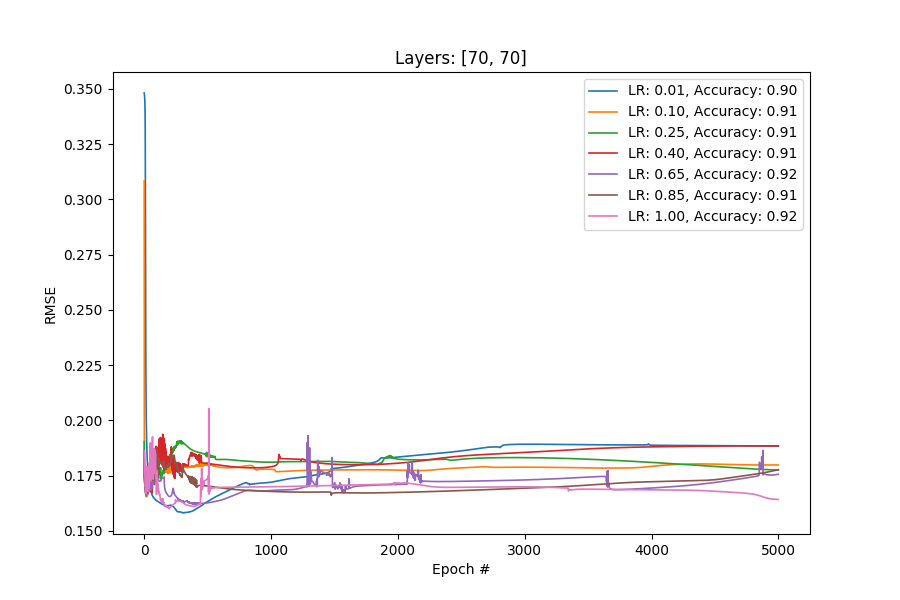
\includegraphics[scale=0.7]{../images/rmse3_20.png} \\}
	     RMSE plot proves that most nets are overfit after 500-1000 epochs.\\
	     
	    It seems like 700 epochs is enough for most networks with 5 layers too.
	    {\center 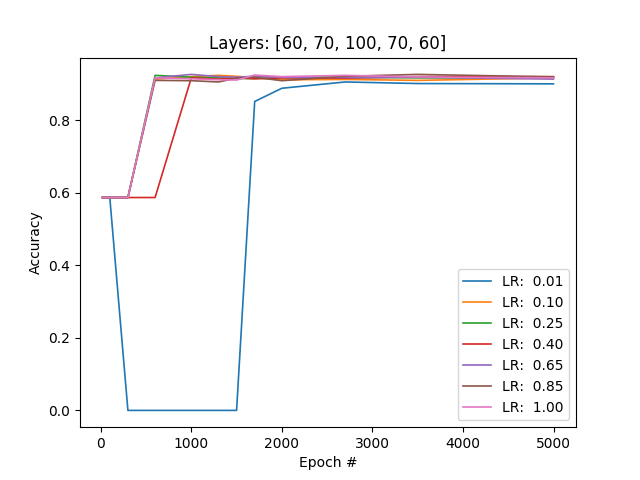
\includegraphics[scale=0.7]{../images/accuracy2_1.png} \\}
	    As we saw before, only net with 0.01 learning rate takes a longer - about 2500 epochs. The highest accuracy value is still around 0.92.
	    RMSE plot shows last accuracy values for 5000 epochs.
	    {\center 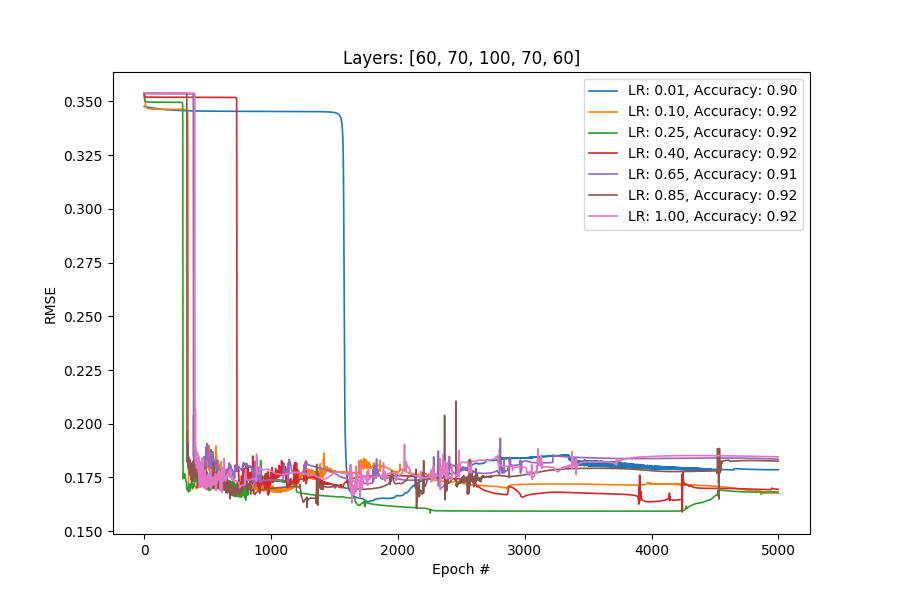
\includegraphics[scale=0.7]{../images/rmse3_1.png} \\}
	    
	    Lastly, I decided to experiment with dimensionality reduction. I chose network with 1 hidden layer with [15] neurons for simplicity. I ran experiment for 500 epochs again only with first 2, 4 and 6 principal components. \\
	    
	    Results definitely don't get better with reducing dimensions to very low values. Here are RMSE plots for 2, 4 and 6 PCAs respectively.
	    {\center 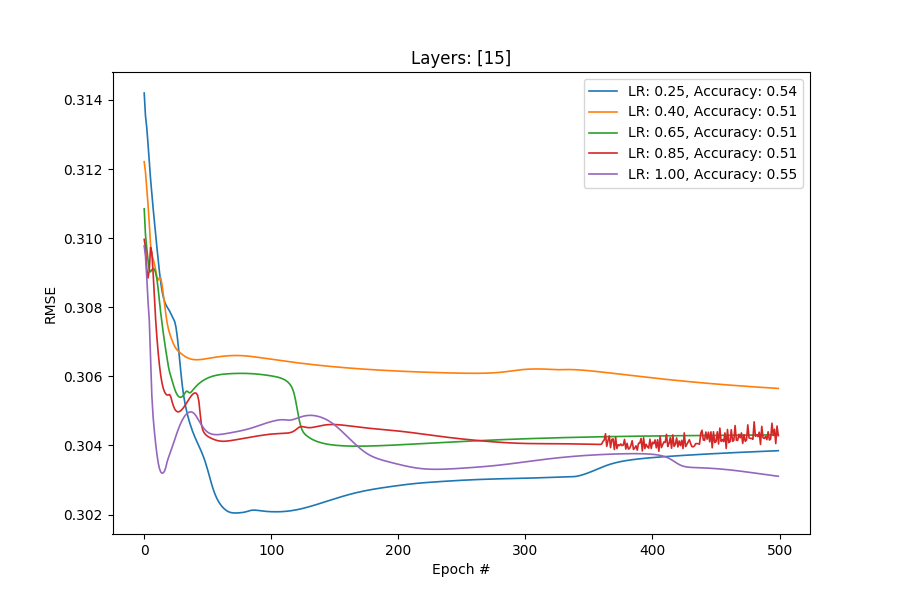
\includegraphics[scale=0.6]{../images/pca_rmse_2.png} \\}
	    {\center 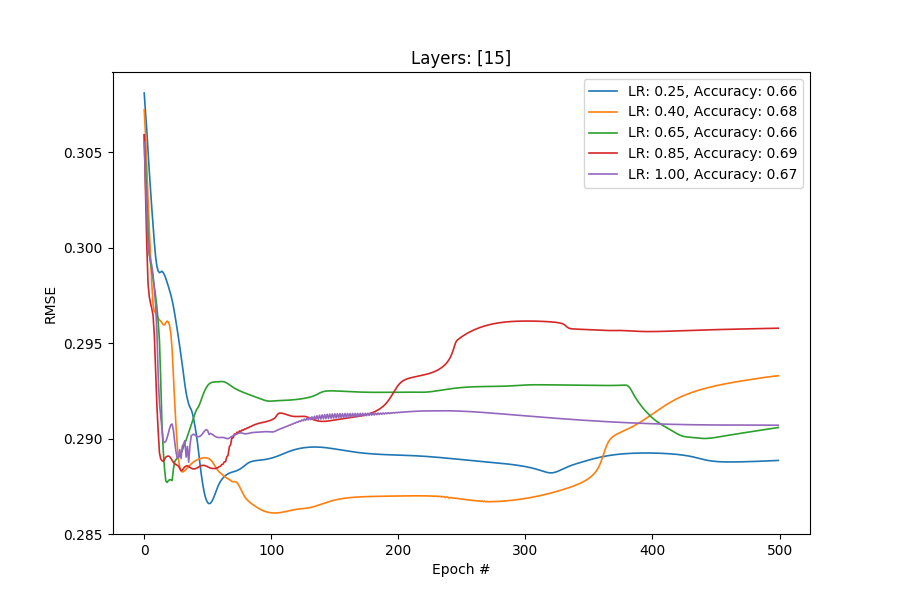
\includegraphics[scale=0.6]{../images/pca_rmse_4.png} \\}
	    {\center 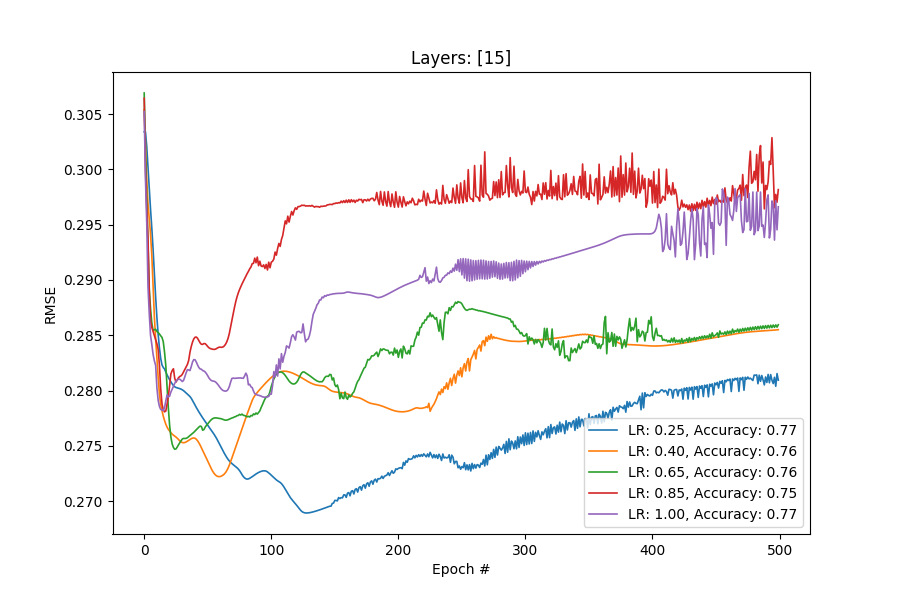
\includegraphics[scale=0.6]{../images/pca_rmse_6.png} \\}
	    
	    We can observe that accuracy grows with number of PCAs. That's how accuracy looks for 6 PCAs for different number of epochs:
	    {\center 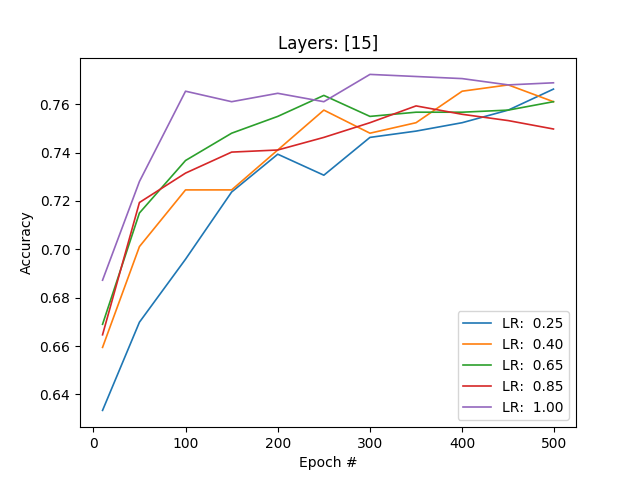
\includegraphics[scale=0.7]{../images/pca_accuracy_6.png} \\}
	    It doesn't get higher than 0.77 and drops for some nets after 350 epochs. So I think we may have too many hidden neurons for 2-6 PCAs, and we also should try more dimensions.
	    
	    SO if we have 30 PCAs, we have better results:
	    {\center 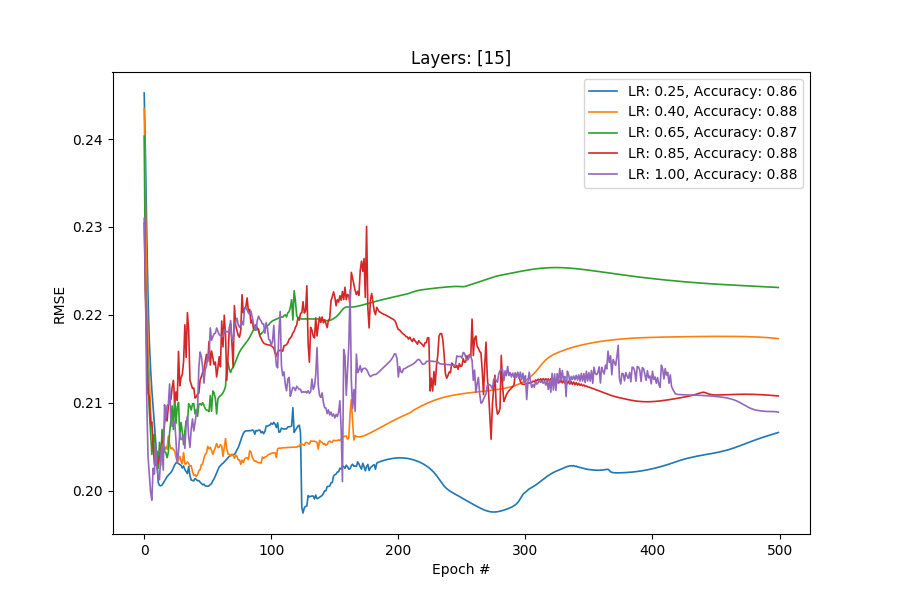
\includegraphics[scale=0.6]{../images/pca_rmse_130.png} \\}
	    Accuracy jumps up to 0.88  for all learning rates I tried. Although we could use less epochs to have values up to 0.90  according to accuracy plot.
	     {\center 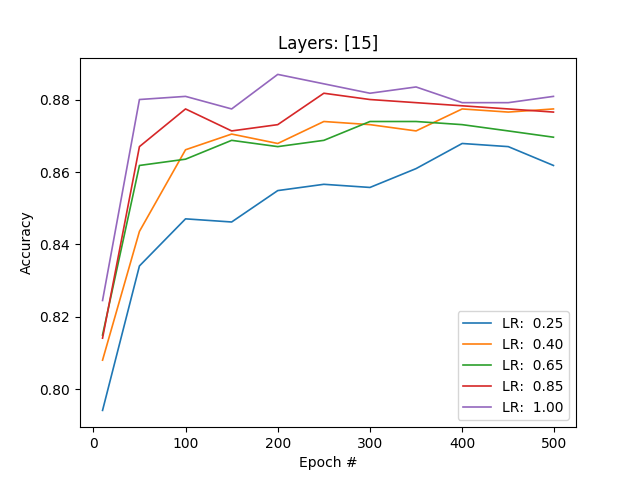
\includegraphics[scale=0.7]{../images/pca_accuracy_130.png} \\}
	     With learning rate of 1.00 we could train net for 200 epochs and achieve good results.
	     
	     I was wrong with reducing number of neurons, instead of increasing number of PCAs. Here is net wit 7 neurons in hidden layer trained for 6 PCAs:
	     {\center 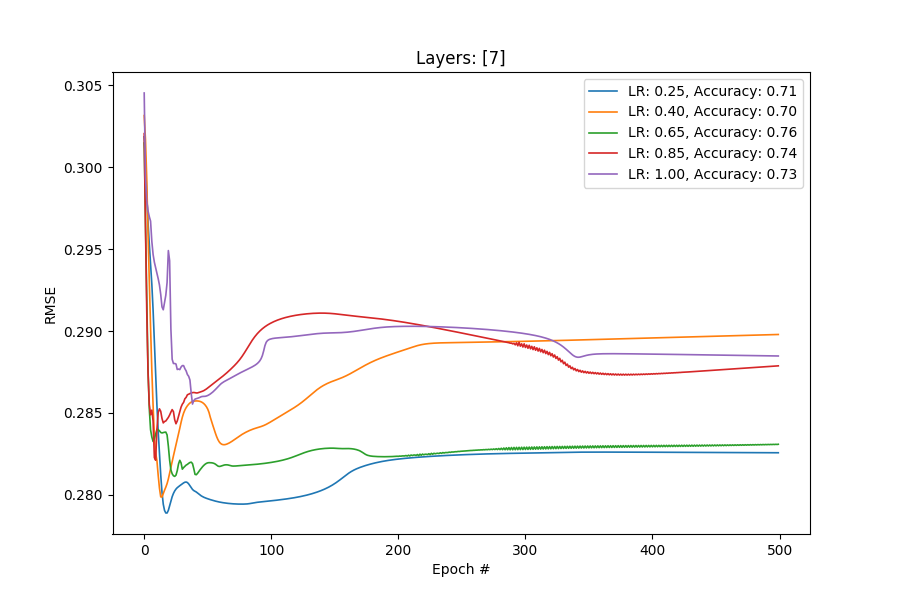
\includegraphics[scale=0.6]{../images/pca_rmse_16.png} \\}
	     Results are not better than with 15 neurons in the layer, they are actually lower. So, I think that larger number of dimensions works better for this type of problem.
	     
	{\bf \item Conclusions.}\\
	
	I've ran several experiments in this project to observe how good we can train neural nets to predict e-mail being spam or not spam. I've tried 1-5 hidden layers and different number of neurons in each: smaller and higher than number of inputs. I've also looked at the performance at different number of epochs. After I could see general results like what number of epochs, layers ,neurons and learning rates are optimal, I ran a few experiments with reduced data. So, for the proportions for splitting data and for the way I decide if e-mail is spam or not, the highest accuracy I could achieve was 0.93, which is not bad. With an RMSE being around 1.7 and plus adding \( \pm \) 0.01 to that, I was pretty much marking data with .8 result value as spam, when I could use higher delta values. Any way, for all runs it seems that higher learning rates give us better performance. It is not necessary to have too many epochs, depending on number of layers 300-700 is optimal. More hidden layers require more epochs to train networks. \\
	Reducing dimensions didn't show great results in my experiment. 30 PCAs was fine, but going down to 2-6 made network perform much worse. \\
	
\end{enumerate}
\end{document}
	
	
	
	
	
	
